\chapter{Revisão Bibliográfica}
\label{revisao_bibliografica}

\section{Figuras}

Para incluir figuras use o seguinte comando:

\begin{figure}[h]
\centering
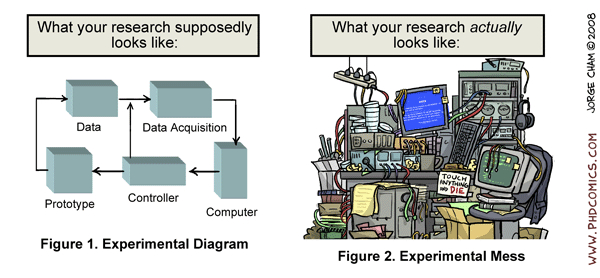
\includegraphics[width=0.6\textwidth]{chapters/fig/research.jpg}
\caption{Legenda da Figura}
\label{label_figura}
\end{figure}

\section{Tabelas}

Pode incluir tabelas usando os ambientes ``table'' + ``tabular'':

\begin{table}[h]
\centering
\caption{Legenda da Tabela usando tabular}
\label{label_tabela_tabular}
\begin{tabular}{||c c c c||} 
\hline
Col1 & Col2 & Col2 & Col3 \\ 
\hline\hline
1 & 6 & 87837 & 787 \\ 
\hline
2 & 7 & 78 & 5415 \\ 
\hline
3 & 545 & 778 & 7507 \\ 
\hline
4 & 545 & 18744 & 7560 \\ 
\hline
5 & 88 & 788 & 6344 \\ 
\hline
\end{tabular}
\end{table}

Também pode usar o ambiente ``table'' e inserir uma tabela como figura:

\begin{table}[h]
\centering
\caption{Legenda da Tabela usando figura}
\label{label_tabela_figura}
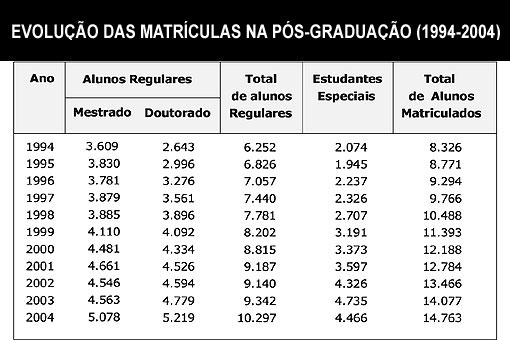
\includegraphics[width=0.5\textwidth]{chapters/fig/tabela.jpg}
\label{label_figura}
\end{table}

\section{Siglas}

Edite o arquivo ``glossary.tex'' com as suas siglas. Veja como exemplo para a sigla do Mestrado Acadêmico em Ciência da Computação da Universidade
Estadual do Ceará.

Este documento é o modelo de qualificação do \acrshort{macc} - \acrshort{uece}

\section{Incluindo referências}

Coloque suas referências no arquivo ``bib.bib'' e cite assim \cite{lamport1986latex}.
